%------------------------------------------------------------------------------%

\subsubsection{Contexto}

\stopcounter
\begin{frame}{Origem}
  O \textbf{Angular Freeze-Tag Problem} (AFTP) surge como um problema de \textbf{\emph{broadcast}} entre satélites em 2018~\cite{Fe18}:
  \bigbreak
  \begin{minipage}{\linewidth}
    \centering
    \colorbox{white}{\multiinclude[format=png, start=0, end=3, graphics={height=4cm}]{AFTP/instance/Temp}}
  \end{minipage}
\end{frame}
\inccounter

\begin{frame}{Motivação}
  \begin{itemize}[<+->]

    \item Recursos limitados restringem o movimento dos satélites;

    \item Grandes distâncias impossibilitam um \emph{broadcast} simultâneo;

    \item O crescimento das constelações de satélites exige protocolos eficientes de transmissão de dados.

  \end{itemize}
\end{frame}

\begin{frame}{Definição - Instância}
  \begin{itemize}[<+->]

    \item Conjunto $P = \{p_1, \dots, p_n\}\subseteq \R^d$ de posições distintas;

    \item Cada $p_i$ corresponde a um satélite associado a $\alpha_i$;

    \item Inicialmente, apenas $p_1$ contém um dado a ser propagado.

  \end{itemize}
\end{frame}

\begin{frame}{Definição - Solução}
  As sequências de rotações onde o objetivo é minimizar o \emph{makespan}:

  \pause

  \bigskip
  \begin{minipage}{\linewidth}
    \centering
    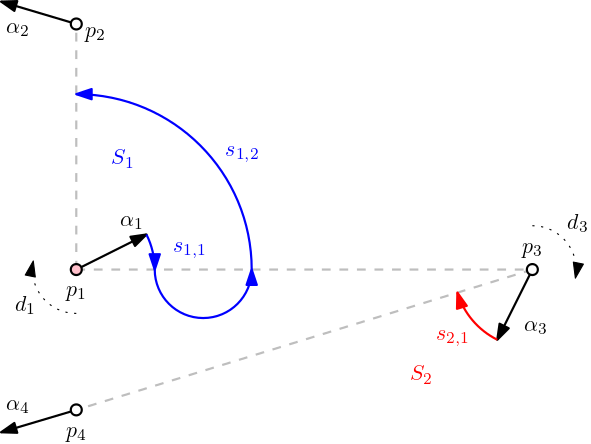
\includegraphics[height=5.5cm]{AFTP/solution.png}
  \end{minipage}
\end{frame}

%------------------------------------------------------------------------------%

\subsubsection{Resultados Teóricos}

\begin{frame}{Resultados Anteriores}
  \begin{thm}[Fekete e Krupke~\cite{Fe18}]
    É NP-difícil aproximar o AFTP em 2D dentro de um fator menor que $\nicefrac{5}{3}$.
  \end{thm}

  \pause

  \begin{thm}[Fekete e Krupke~\cite{Fe18}]
    Existe uma $9$-aproximação para o AFTP em 2D, assumindo um limite inferior de $\varepsilon>0$ para a rotação inicial de qualquer satélite que rotacione sua antena.
  \end{thm}
\end{frame}

\begin{frame}{Nossos Resultados}
  \setbeamercolor{block body}{bg=green!35!white}
  Chamamos de \textbf{energia total} de uma solução a soma da rotação total realizada por todos os satélites.

  \pause

  \begin{thm}
    Seja $I$ uma instância do AFTP em 2D, $E$ um número real e $k$ um inteiro positivo.
    %
    Então, existe um algoritmo que roda em tempo ${(n\frac{Ek}{\varepsilon})^{O(\frac{Ek}{\varepsilon})}}$ e ou prova que toda solução ótima requer mais de $E$ de energia total, ou encontra uma solução com \emph{makespan} no máximo ${(1+\nicefrac{1}{k})\opt(I)}$.
  \end{thm}

  \pause

  \begin{thm}
    Para todo inteiro positivo $k$, existe uma \mbox{$(1+\nicefrac{1}{k})$-aproximação} para o AFTP em 2D com o objetivo de minimizar a energia total, que roda em tempo \mbox{$(n\frac{k}{\varepsilon})^{O(\frac{k}{\varepsilon})}$}.
  \end{thm}
\end{frame}
